\documentclass[12pt,letterpaper]{article}
\usepackage[latin1]{inputenc}
\usepackage{xcolor}
\usepackage{pstricks}
\usepackage{graphicx}
\usepackage[spanish]{babel}

\begin{document}

{\Huge {\rm { \bf Instituto Politecnico Nacional}}}\\
\begin{center}
{\huge {\rm {\em Escuela Superior de C\'omputo}}} \\
\end{center}
\begin{center}
{\Large {\em Tecnolog\'ias para la Web}}\\
\end{center}
\begin{center}
{\Large Alejandro Hern\'andez Hern\'andez}\\
\end{center}
\begin{center}
{\huge {\bf PR\'ACTICA 1}}
\end{center}


\newpage
{\Huge {\rm {\bf Introducc\'ion}}}
\\

El {\em lenguaje de marcado extensible (XML)}, es un lenguaje que permite el almacenamiento y transporte de datos. Es muy similar a html, solo que XML es mas estricto, y su funcion radica en escribir datos y no mostrarlos como HTML.\\
\vspace{2mm}
{\tiny {\verb@referencia:https://www.w3c.es/Divulgacion/GuiasBreves/TecnologiasXML ; https://www.w3schools.com/xml/xml_whatis.asp @}}
\\

Dentro del contexto de XML, tenemos, ademas de los archivos con extension XML, los {\em Data Type Definition} ({\em DTD}, definicion de tipos de datos), en los cuales se nombran los elementos que se utilizar\'an en un archivo XML, en otras palabras, los DTD son la definicion de las etiquetas a usar. \\En esta practica, se realiz\'o un ejemplo de archivo XML y un DTD, ambos con la etiqueta persona, y el DTD definiendo los campos del mismo.  

\newpage
{\Huge {\rm {\bf Desarrollo}}}
Lo primero a realizar, es la definicion en un esquema de laetiqueta persona, es decir, los elementos que definen a una persona.
\\La abstracci\'on que se realiz\'o fue la siguiente: 
\begin{center}
\fboxsep 12pt
\begin{minipage}[t]{6cm}
{ una persona tiene:
\begin{itemize}
\item nombre
\item apellido paterno
\item apellido materno
\item direccion
\item codigo postal
\item edad
\item estado donde radica
\item curp
\item fecha de nacimiento
\item telefono
\end{itemize}
}
\end{minipage}
\end{center}
Por lo tanto, nuestro DTD quedar\'ia como: \\
\vspace{1cm}
\begin{minipage}[t]{8cm}
{
\begin{verbatim}
<?xml version="1.0" encoding="UTF-8"?>
<!DOCTYPE persona[
<!ELEMENT persona (nombre*,apellidoPat+,apellidoMat+,direccion,
cp,edad,estado,curp+,fechaNac,telefono)>
<!ELEMENT nombre (#PCDATA)>
<!ELEMENT apellidoPat (#PCDATA)>
<!ELEMENT apellidoMat (#PCDATA)>
<!ELEMENT direccion (#PCDATA)>
<!ELEMENT cp (#PCDATA)>
<!ELEMENT edad (#PCDATA)>
<!ELEMENT estado (#PCDATA)>
<!ELEMENT curp (#PCDATA)>
<!ELEMENT fechaNac (#PCDATA)>
<!ELEMENT telefono (#PCDATA)>
]>
\end{verbatim}

}
\end{minipage}

Ahora, un ejemplo de la implementacion de la etiqueta persona ser\'ia:
%\vspace{5mm}
\begin{minipage}[t]{8cm}{
\vspace{2mm}
\begin{verbatim}
<persona>
<nombre>Alejandro</nombre>
<apellidoPat>Hernandez</apellidoPat>
<apellidoMat>Hernandez</apellidoMat>
<direccion>eso es algo que no revelare</direccion>
<cp>56020</cp>
<edad>21</edad>
<estado>Mexico</estado>
<curp>HEHA950213HMCRRL15</curp>
<fechaNac>13-02-1995</fechaNac>
<telefono>5569874123</telefono>
</persona>
\end{verbatim}
}
\end{minipage}
\\

\vspace{5mm}
Luego, tenemos 2 formatos para poder ocuparlo:\\
1. que se importe el DTD al XML, o\\
2. que se defina la etiqueta persona en el archivo XML
\\

Como debemos validar o comprobar que nuestro DTD y XML sean correctos, se opt\'o por la $2^a$ opci\'on.
\\
Por lo tanto, nuestro archivo final queda como:

\begin{minipage}[t]{8cm}
{
\begin{verbatim}

<?xml version="1.0"?>
<!DOCTYPE persona[
<!ELEMENT persona (nombre*,apellidoPat+,apellidoMat+,direccion,
cp,edad,estado,curp+,fechaNac,telefono)>
<!ELEMENT nombre (#PCDATA)>
<!ELEMENT apellidoPat (#PCDATA)>
<!ELEMENT apellidoMat (#PCDATA)>
<!ELEMENT direccion (#PCDATA)>
<!ELEMENT cp (#PCDATA)>
<!ELEMENT edad (#PCDATA)>
<!ELEMENT estado (#PCDATA)>
<!ELEMENT curp (#PCDATA)>
<!ELEMENT fechaNac (#PCDATA)>
<!ELEMENT telefono (#PCDATA)>
]>


<persona>
<nombre>Alejandro</nombre>
<apellidoPat>Hernandez</apellidoPat>
<apellidoMat>Hernandez</apellidoMat>
<direccion>eso es algo que no revelare</direccion>
<cp>56020</cp>
<edad>21</edad>
<estado>Mexico</estado>
<curp>HEHA950213HMCRRL15</curp>
<fechaNac>13-02-1995</fechaNac>
<telefono>5569874123</telefono>
</persona>

\end{verbatim}
}
\end{minipage}
\newpage
Y lo llamaremos {\em persona.xml}. Luego, nos dirigimos a la pagina web :\\{\em https://www.xmlvalidation.com/} \\y nos aparecer\'a:
\begin{center}
\begin{figure}[h]
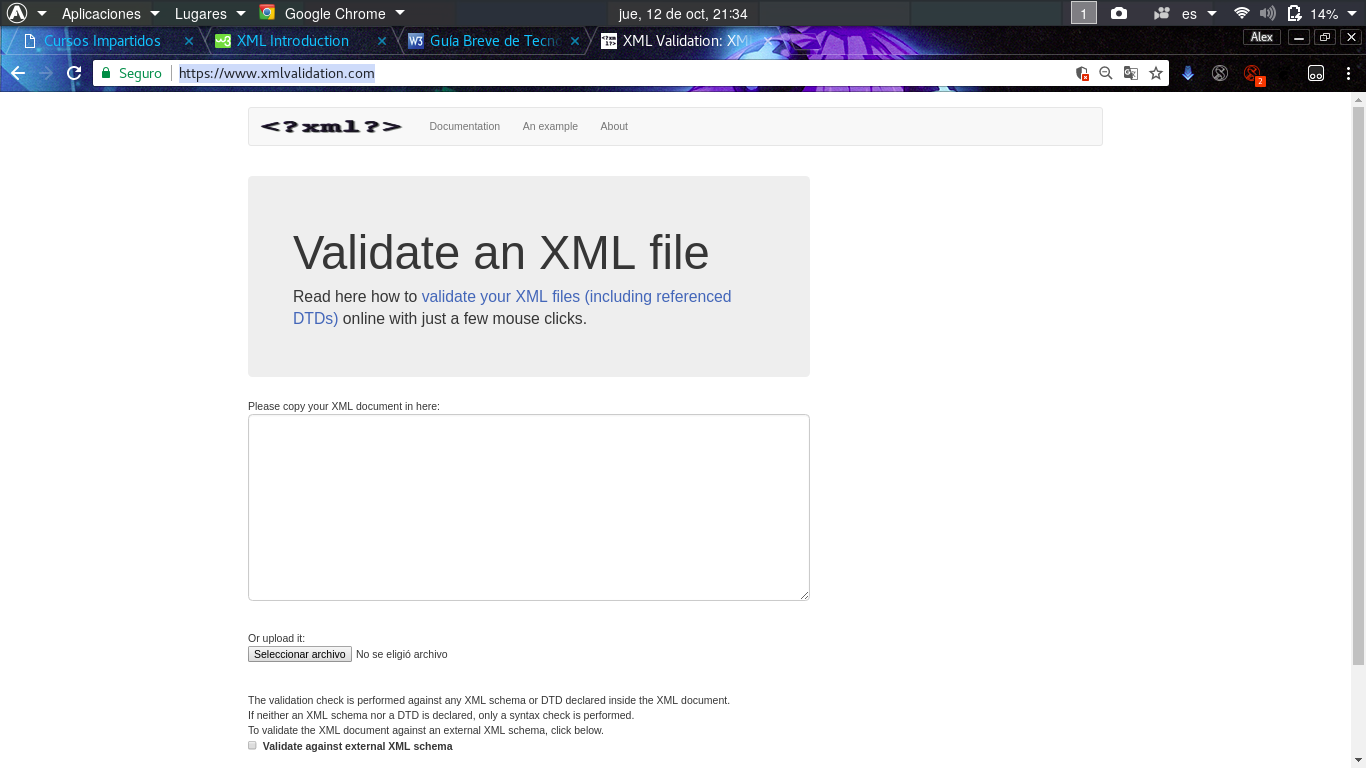
\includegraphics[width=400pt]{./imgs/xlmval.png}
\vspace{-2mm}
\caption{Validador xml}\label{figure 1}
\end{figure}
\end{center}
\newpage


y en la caja de texto ingresamos el codigo xml:

\begin{center}
\begin{figure}[h]
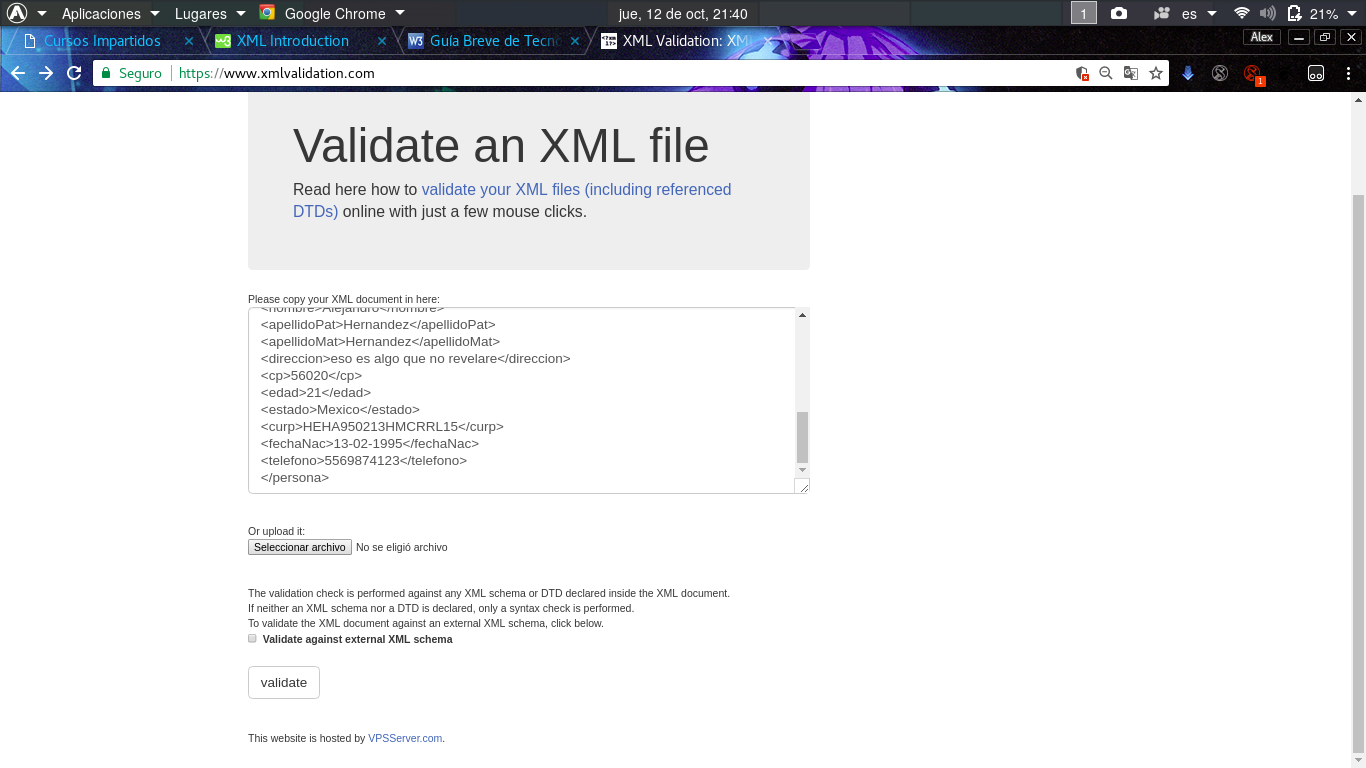
\includegraphics[width=400pt]{./imgs/codigo.png}
\vspace{-2mm}
\caption{Validador xml con codigo}\label{figure 1}
\end{figure}
\end{center}
\vspace{3mm}
\newpage

damos click en ``validar"\ y si no hay errores se muestra: 

\begin{center}
\begin{figure}[h]
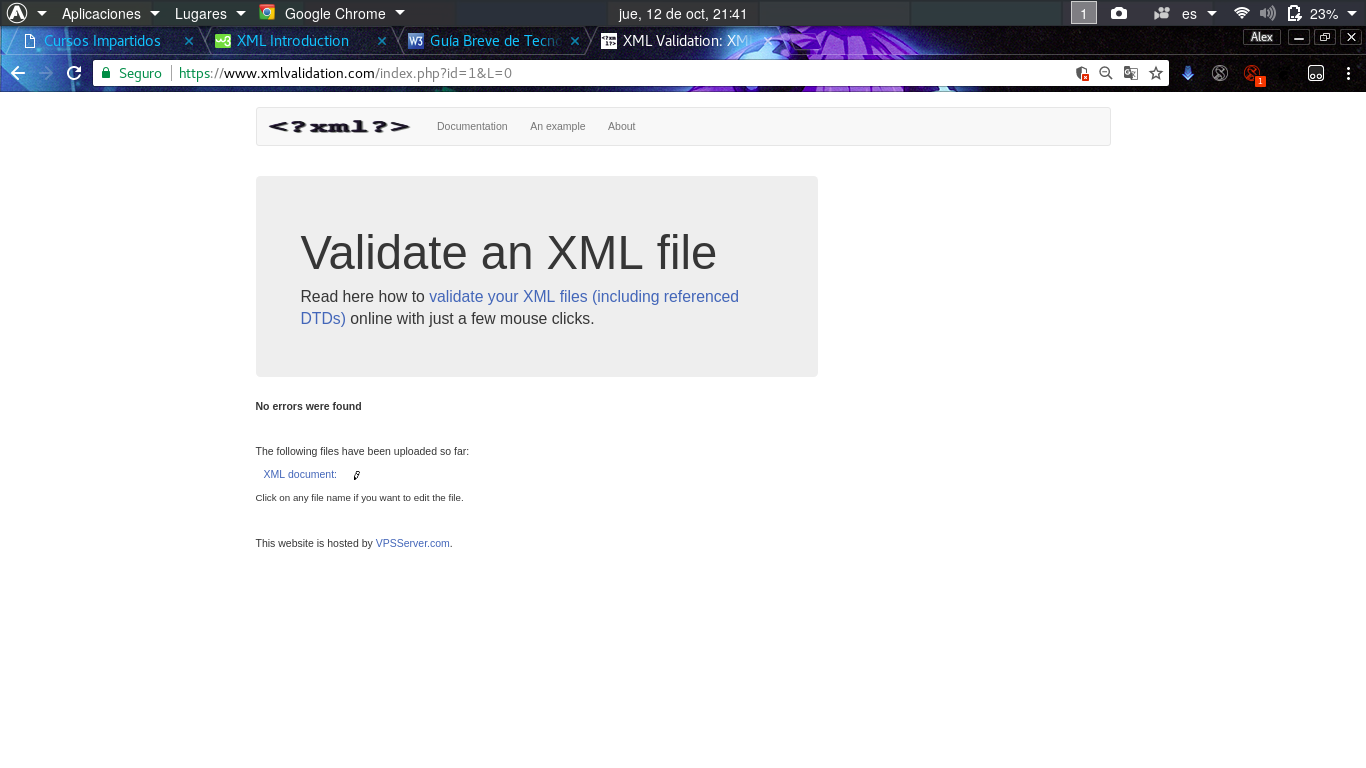
\includegraphics[width=400pt]{./imgs/validado.png}
\vspace{-2mm}
\caption{codigo validado}\label{figure 1}
\end{figure}
\end{center}

\newpage
{\Huge {\rm {\bf Conclusi\'on}}}

\vspace{5mm}
La ventaja de xml es que nos permite definir las etiquetas ``a nuestro antojo", porque podemos darle el nombre que querramos, y con esta practica, queda demostrado, pues se defini\'o un elemento {\em persona} y se definieron sus componentes.
\\Asi, podemos ver que XML es un lenguaje de marcado poderoso y facil de implementar, ademas de poder definir los elementos en el mismo archivo {\em xml} o importarlo desde un archivo {\em DTD} a un {\em xml}.


%fin documento
\end{document}
